\documentclass{article}
\usepackage{enumitem}
\usepackage{gensymb}
\usepackage[normalem]{ulem}
\usepackage{fixltx2e}
\usepackage{color}
\usepackage[hidelinks]{hyperref}
\usepackage{graphicx}
\usepackage[top=2cm,bottom=2cm,left=3cm,right=3cm]{geometry}
\usepackage{multicol}
\usepackage{float}

\usepackage{wrapfig}
\usepackage{supertabular}
\usepackage{supertabular,booktabs}



\begin{document}
    \section{Experimental Results}
	In order measure performance and to best guide the design choices available, we conducted several experiments on the key components of the task. This section details and discusses the methods, results, and implications of the testing.

	\subsection{Odometry Noise}
	The Pioneer P3-DX robot is subject to marginal noise in its odometry readings. Discrepancies in the reported position of the robot from the localisation algorithm versus the reported position from the odometer give an indication of the level of noise to expect (and thus to account for). It should be noted, however, that our testing was subject to human error. Eliminating this error vector would have demanded more complex testing methods stretching beyond the scope of the exercise.

The motor of the Robot has a short delay before starting. We tested this to be consistent at~2 seconds (+- 0.1) and accounted for it in any movement-based tests by initializing the motor (by sending a spurious non-movement command) prior to sending a movement command.

	\subsubsection{Translation Noise}
	The translation noise was measured by driving the robot forwards with a set velocity and time. The results of the 30 test instances indicated that the translation noise was on average ~0.7\%, with this value fairly consistent across a variety of time values when using a value of 0.25 for speed.
	\begin{figure}[H]
	\begin{center}
	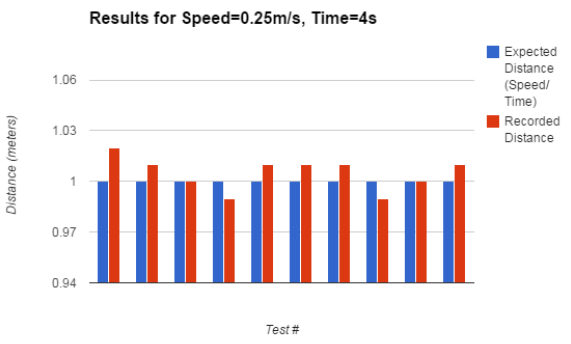
\includegraphics[width=0.9\linewidth]{ExperimentalResults1}
	\caption{Translation noise test 1}
	\end{center}
	\end{figure}
	\begin{figure}[H]
	\begin{center}
	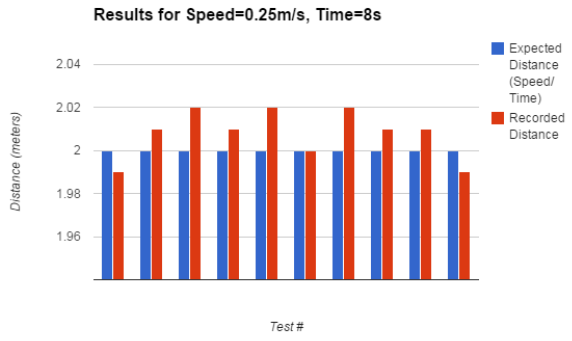
\includegraphics[width=0.9\linewidth]{ExperimentalResults2}
	\caption{Translation noise test 2}
	\end{center}
	\end{figure}
	\begin{figure}[H]
	\begin{center}
	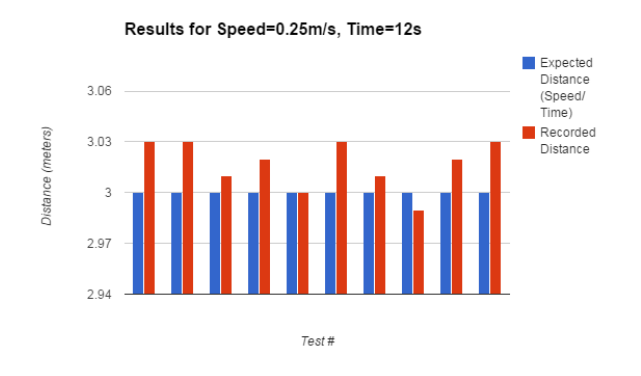
\includegraphics[width=0.9\linewidth]{ExperimentalResults3}
	\caption{Translation noise test 3}
	\end{center}
	\end{figure}
	
	\subsubsection{Drift Noise}
	Drift noise levels were calculated by instructing the Robot to drive 1, 2, or 3 meters on a predefined straight path, and then measuring the x-axis deviation from that path, repeating the process 20 times for each distance.

Our results showed an average drift per meter of 2.9159 cm/m for the 60 tests at the 3 different distances (2.7125, 2.99 and 3.045 for 3 meters, 2 meters, and 1 meter respectively). This means that for each meter the robot drives forwards, it will on average drift ~2.9159cm. The results also suggest that the drift noise decreases (in relative terms) as distance increases. Further testing would be required to test this hypothesis, however, as our results could be specific to the distances we tested (i.e. the phenomena is only observable over small distances <= 3 meters), or simply anomalous to our small data set of 60 test instances. Figures 4.2 shows the results.
	
	\begin{figure}[H]
	\begin{center}
	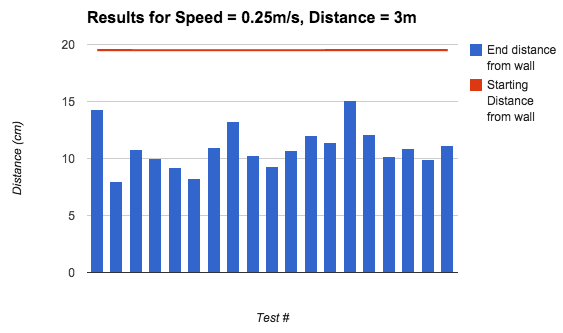
\includegraphics[width=0.9\linewidth]{ExperimentalResults4}
	\caption{Drift noise test 1}
	\end{center}
	\end{figure}
	\begin{figure}[H]
	\begin{center}
	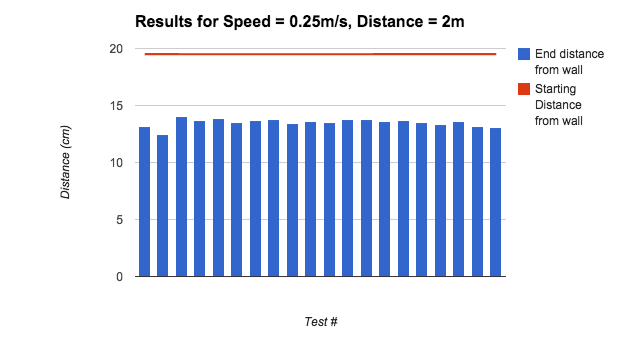
\includegraphics[width=0.9\linewidth]{ExperimentalResults5}
	\caption{Drift noise test 2}
	\end{center}
	\end{figure}
	\begin{figure}[H]
	\begin{center}
	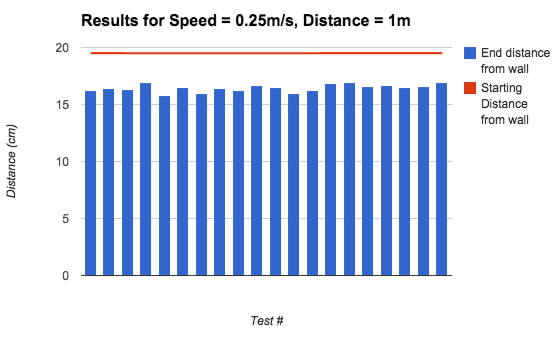
\includegraphics[width=0.9\linewidth]{ExperimentalResults6}
	\caption{Drift noise test 3}
	\end{center}
	\end{figure}
	
	\subsubsection{Rotation Noise}
	To test rotation noise we set the Robot to turn a set value, pi radians (180 degrees), at a set angular.z velocity (turning speed) of 4/pi radians/second (meaning it was turning at 45 degrees/second). The actual number of degrees turned over the 4 seconds was then measured and the difference compared. Over 30 test instances the average difference was found to be ~00.55\% with a variance of +-4 degrees.
	\begin{figure}[H]
	\begin{center}
	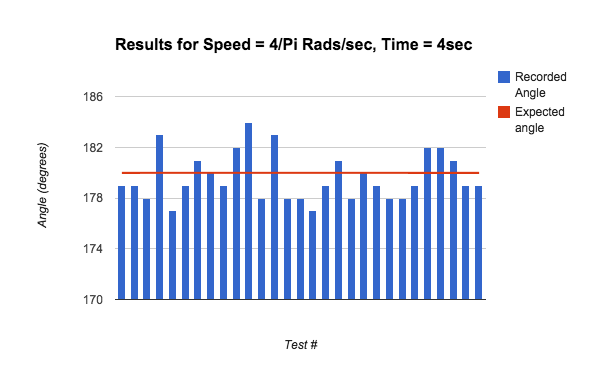
\includegraphics[width=0.9\linewidth]{ExperimentalResults7}
	\caption{Rotation noise test 1}
	\end{center}
	\end{figure}
	
	\subsection{Localisation Performance}
	Whilst we adopted the ACML localisation as part of the ROS package over a bespoke MCL implementation we had previously developed, we still tested our bespoke implementation for its robustness, and whether it could indeed be successfully used in a non-trivial application. Both localisation methods were analysed by the speed at which they could localise the robot as it travelled to a pre-set point. For the sake of brevity, the testing was conducted in the stage simulation.

Our results (Figure 4.4) show that the ACML implementation outperforms our MCL implementation significantly (~35\% quicker in achieving localisation) and with a smaller deviation in the results (a standard deviation of ~4.06 versus ~5.81). Our MCL implementation, however, always succeeded in localising the robot, and time constraints notwithstanding, could be used in place of the ACML implementation.
	\begin{figure}[H]
	\begin{center}
	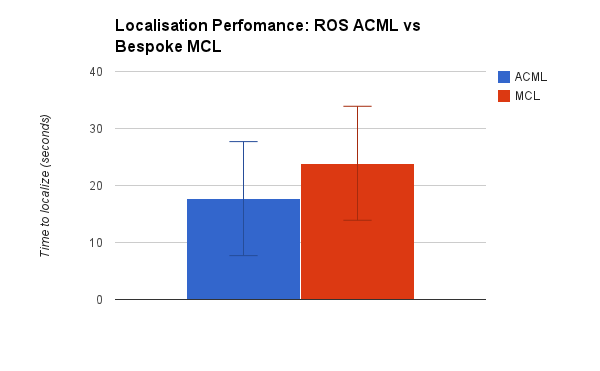
\includegraphics[width=0.9\linewidth]{ExperimentalResults8}
	\caption{Performance of ROS ACML vs our bespoke ACML implementation}
	\end{center}
	\end{figure}
	
	
	
	
	
	\subsection{Exploration}
	We tested two possible exploration strategies for our robot. One strategy was allowing the robot to free roam and the other was setting a fixed path through hard-coded points.
	
      \subsubsection{Random Exploration}
   To test the feasibility of the random navigation strategy we allowed the robot to freely roam across the floor. In free roaming it discovered more areas, and in more detail, than the specific point navigation strategy. However, as seen from Figure 9, the exploration is stochastic and inefficient: the robot often looped back on itself, at times circling for several minutes.
  \begin{figure}[H]
	\begin{center}
              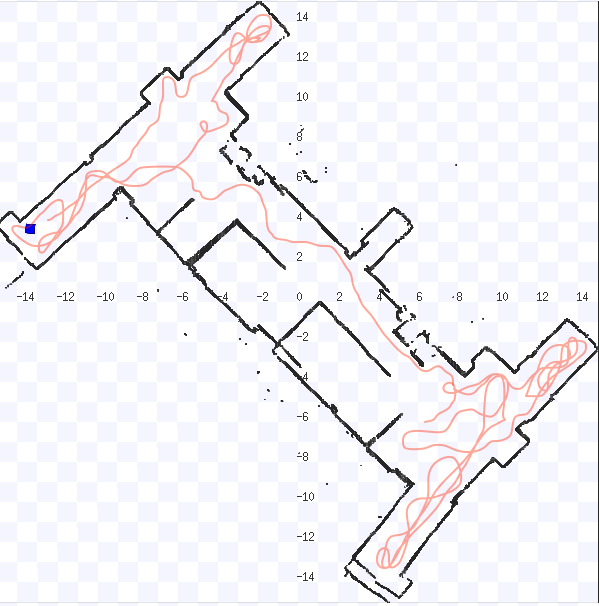
\includegraphics[width=0.8\linewidth]{ExperimentalResults9}
	\end{center}
              \caption{Random exploration route}
          \end{figure}
          
      \subsubsection{Specific Point Exploration}
   In the specific point exploration strategy we gave our robot 6 points in which to roam. Though significantly reducing the overall exploration range, it did make identifying people much faster, as only those map regions with high likelihood to have a person were explored and areas such as corners ignored. Additionally, the robot did not loop back on itself or otherwise behave inefficiently. We selected this strategy in our implementation.

          \begin{figure}[H]
	\begin{center}
              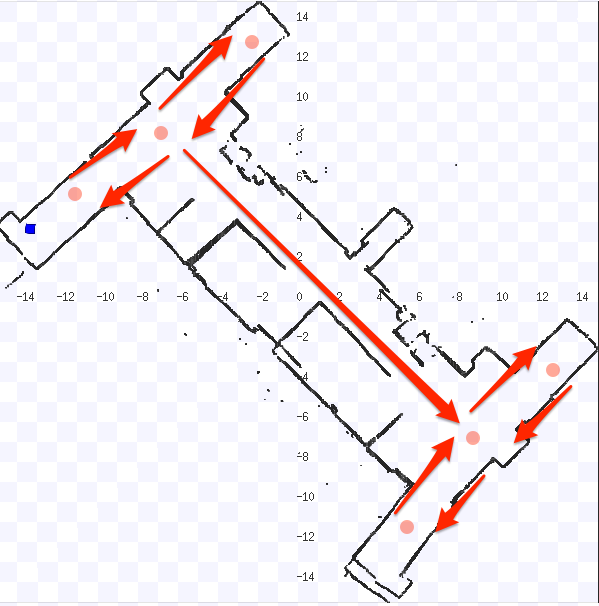
\includegraphics[width=0.8\linewidth]{ExperimentalResults10}
              \end{center}
              \caption{Plotted exploration route}
          \end{figure}
	
	\subsection{Human Detection Testing}
	\subsubsection{Leg Detector Average}
	To measure the best value for the leg detector average we let the robot roam along a set path using the navigation stack as the driver, recording the averages calculated from the number of legs detected/the number of readings taken. This provided an average value to increase the effectiveness of our leg detection. We measured and modified the amount of readings taken before calculating the average and the threshold value to cause the Robot to believe a person was present to find the most suitable parameters for the task.

	\begin{supertabular}{r | p{2cm} | p{2.5cm} | p{8cm} }
	Test & Average number & Amount of Readings taken & Observed Result \\
	\hline
	  &  &  \\[2ex]
	1 & 0.5 & 50000 & Many False Positives :Robot thinks people are there when they are not. \\[1ex]
	2 & 0.5 & 100000 & Many False Positives: Robot thinks people are there when they are no. Average is lower. \\ [1ex]
3 & 0.5 & 150000 & Many False Positives: Robot thinks people are there when they are not, but average is lower again. Average appears to be too low. \\ [0ex]

	  &  &  \\[2ex]
4 & 0.75 & 50000 & Less false positives, but average does not differ too much when someone is in front of the Robot \\[1ex] 
5 & 0.75 & 100000 & Very similar to test \#4, but more responsive when used with more readings. Average may need to be increased. \\ [0ex]
6 & 0.75 & 150000 & Again very similar to test \#4, but taking too long between each assumption. \\ [1ex]

	  &  &  \\[2ex]
7 & 1 & 50000 & Detected the legs and low positives. Average consistently higher due to low number of readings taken \\ [1ex]
8 & 1 & 100000 & Timely and  accurate assumption. \\ [2ex]
9 & 1 & 150000 & Low false positives but took too long between readings and would sometimes overshoot people while driving. \\ [1ex]

	  &  &  \\[2ex]
10 & 1.25 & 50000 & Higher average decreased the false positives but meant that if no false positives were detected then the average would not be above the threshold. \\ [0ex]
11 & 1.25 & 100000 & A higher number of readings seemed to decrease the average number further, no detections if there are no false positives. \\ [0ex]
12 & 1.25 & 150000 & A higher number of readings seemed to decrease the average number further, no detections if there are no false positives.  \\[0ex] 

	  &  &  \\[2ex]
13 & 1.5 & 50000 & Significantly less false positives, higher average seems to lead to less humans being falsely detected. \\ [1ex]
14 & 1.5 & 100000 & The higher number of readings meant the average was lower. It rarely reached over the threshold. \\ [1ex]
15 & 1.5 & 150000 & The higher number of readings meant the average was lower. It rarely reached over the threshold. \\[1ex]
	
	\end{supertabular}
	
	
	Based on the experimental data we chose to use 100,000 readings with an average of 1. This gave us the most accurate detection rate that someone was present whilst also performing in a reasonable amount of time. Using more readings, whilst producing a more accurate result, would not have yielded a timely enough result. The average of ‘1’ means that the robot has to have seen at least one person during the entirety of its scan. This dramatically reduced the false positive rate while exploring; whilst the leg detector might produce false positives at a given point it is unlikely to detect it over its entire scan.

\columnbreak
\vspace*{20.5cm}

	\subsubsection{Leg Detector Parameters}
	To determine the best parameters for the Leg Detection algorithm (largely to eliminate the large number of false positives which it originally suffered), we placed the robot in a fixed, stationary position, looking in to a corridor (the most controlled setting we could find). We then ran our tests, first seeing if the values detected any false positives. We then changed the values to try and reduce these false positives and then introduced a person into the scanners range to check that they were accurately detected.
	
\begin{supertabular}{r|r|r|r|r|r|p{8cm}}
AMin & AMax & BMin & BMax & CMin & CMax & Observed Result\\
\hline
 & & & & & & \\

0.1 & 0.2 & 0 & 0.4 & 0.1 & 0.4 & Robot seemed very sensitive, was set off by many obstacles.\\

 & & & & & & \\
 0.1 & 0.15 & 0 & 0.4 & 0.1 & 0.4 & This seemed to have no effect, still very sensitive.\\[1ex]
 0.1 & 0.3 & 0 & 0.4 & 0.1 & 0.4 & This seemed to increase the number of false positives detected.\\
 0.05 & 0.2 & 0 & 0.4 & 0.1 & 0.4 & This increased the number of false positives detected.\\[1ex]
 0 & 0.2 & 0 & 0.4 & 0.1 & 0.4 & This dramatically increased the number of false positives detected\\
 0.1 & 0.2 & 0 & 0.4 & 0.1 & 0.4 & These values seem to yield the best results.\\ [1ex]
 & & & & & & \\ 
 0.1 & 0.2 & 0.2 & 0.4 & 0.1 & 0.4 & This did not reduce the false positives at all.\\[1ex]
 0.1 & 0.2 & 0.1 & 0.4 & 0.1 & 0.4 & This did not reduce the false positives at all.\\[1ex]
 0.1 & 0.2 & 0 & 0.3 & 0.1 & 0.4 & Reduction in false positives, specifically the doorway posts.\\
 0.1 & 0.2 & 0 & 0.2 & 0.1 & 0.4 & No longer detected people as well, missed people standing in a 'normal' pose.\\
 0.1 & 0.2 & 0 & 0.3 & 0.1 & 0.4 & These values seem to yield the best results.\\ [1ex]
 & & & & & & \\
 0.1 & 0.2 & 0 & 0.3 & 0.2 & 0.4 & Did not seem to affect the number of false positives.\\[1ex]
 0.1 & 0.2 & 0 & 0.3 & 0.3 & 0.4 & Did not seem to affect the number of false positives.\\[1ex]
 0.1 & 0.2 & 0 & 0.3 & 0.3 & 0.5 & Did not seem to affect the number of false positives.\\[1ex]
 0.1 & 0.2 & 0 & 0.3 & 0.35 & 0.4 & Did not seem to affect the number of false positives.\\[1ex]
 
 0.1 & 0.2 & 0 & 0.3 & 1000 & 1000 & This is to stop it having an effect at all. These seems to make the robot a lot more reliable.\\
 \end{supertabular}
 
	The parameters we chose are highlighted in bold with qualitative justification presented in the observed result column. After our tests were complete we ran the robot through the full program to check that these results behaved as expected in the viva environment.
	
	\subsubsection{Leg Detector detection rate}
	The leg detection rate was a binary pass:fail test. We set the robot at a static point looking into a room and then have it scan for a person in that room, measuring the number of correct (detecting a person when a person is present or vice versa) and incorrect results.
	\begin{figure}[H]
	\begin{center}
	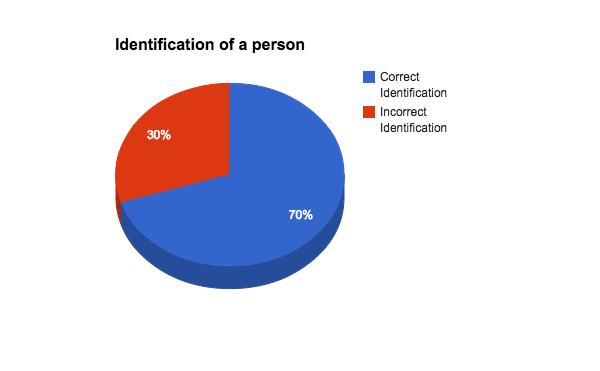
\includegraphics[width=0.8\linewidth]{ExperimentalResults11}
	\caption{Leg detector detection rate of person}
	\end{center}
	\end{figure}


\columnbreak
\vspace*{12.5cm}	
	
	The leg detection yielded an accuracy rate of ~70 percent. We feel this rate is acceptable given the environment of the room and the way the leg detector algorithm works. Nevertheless, we decided that we needed human confirmation (a button press) that a human was genuinely in the room.
	
	\subsection{Obstacle Detection}
	To test the accuracy of the obstacle detection we ran the robot through a set route, placing a wooden board across the path at different points.
	\begin{figure}[H]
	\begin{center}
	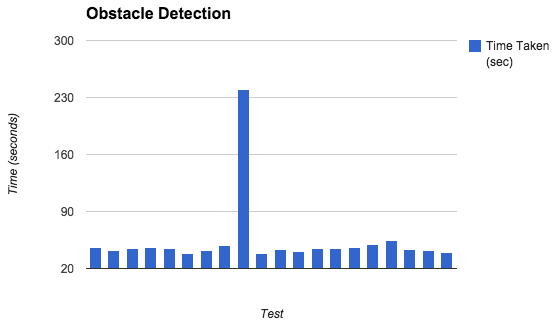
\includegraphics[width=0.8\linewidth]{ExperimentalResults12}
	\caption{Leg detector detection rate of person}
	\end{center}
	\end{figure}
	As evidenced by Figure x, 98\% of the time the robot avoided the board. Difficulties in avoidance arose when the robot became 'trapped' in a corner created by the board and walls.
	
	\subsection{Overall Performance Testing}
	The overall performance tests were ‘full-run’ tests scored by a binary pass:fail metric. Over 10 test instances the Robot robustly succeeded in the full run 8 times. 
	\begin{figure}[H]
	\begin{center}
	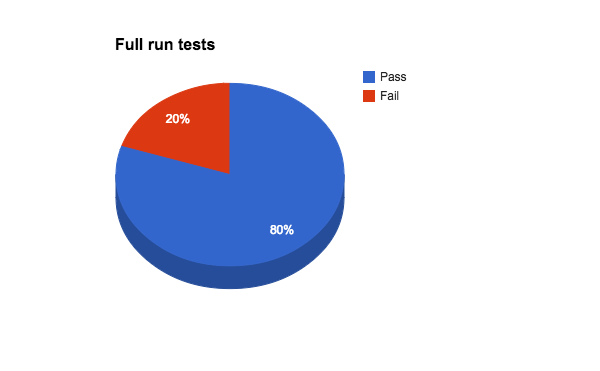
\includegraphics[width=0.8\linewidth]{ExperimentalResults13}
	\caption{Leg detector detection rate of person}
	\end{center}
	\end{figure}
	The feedback from the full-run tests was reassuring; the tests completed successfully 80\% of the time. The reasons for the tests failing were one instance of an object entering the domain and the robot failing to stop in time as it was going too fast (subsequently fixed). The second time the robot got 'stuck' in a corner which, given enough time, we believe it may have eventually worked its self free.
\end{document}